\documentclass{standalone}
\usepackage{tikz}
\begin{document}
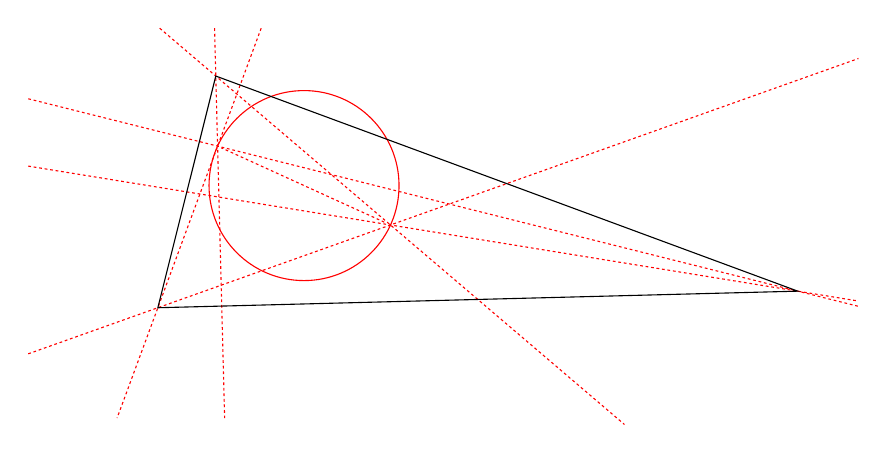
\begin{tikzpicture}[x=1pt,y=1pt]
\draw[red] (99.66,-56.86) circle (34.33);
\draw[red, dash pattern=on 1pt] (67.33,-0.00) -- (70.97,-140.86);
\draw[red, dash pattern=on 1pt] (84.18,-0.00) -- (32.11,-140.86);
\draw[red, dash pattern=on 1pt] (0.00,-25.50) -- (300.00,-100.50);
\draw[red, dash pattern=on 1pt] (0.00,-117.66) -- (300.00,-10.94);
\draw[red, dash pattern=on 1pt] (0.00,-49.82) -- (300.00,-98.58);
\draw[red, dash pattern=on 1pt] (47.51,-0.00) -- (215.45,-143.19);
\draw[red, dash pattern=on 1pt] (128.64,-70.06) -- (69.79,-43.23);
\draw (46.84,-101.00) -- (67.78,-17.28) -- (278.07,-95.01) -- cycle;
\end{tikzpicture}
\end{document}
